\documentclass{article}

\usepackage{amsmath}
\usepackage{graphicx}
\usepackage{float}
\usepackage{bm}
\usepackage{url}
\usepackage[utf8]{inputenc}
\usepackage[margin=2cm]{geometry}
\setlength\parindent{0pt}

\begin{document}

\title{An investigation into the Ethereum Cryptocurrency through Principal Component Analysis}
\author{Andrew P Talbot 1434667}
\date{\today}
\maketitle

\vspace{5mm}
\section{Introduction}
Recently, we have seen the words 'blockchain' and 'cryptocurrency' become real buzzwords, the most famous implementation of this is Bitcoin. This is currently the number one valued cryptocurrency both in price per coin, and total investment into the coin. Bitcoin is a decentralized currency that allows its users to send money using only their computer. It was created by an unknown person under the name of Satoshi Nakamoto, and since its creation we have seen plenty of new coins, and a community of people passionate about the technology that it provides, and other people interested in the opportunity that it's volatile market offers. This project however focuses on the current second largest cryptocurrency, which is Ethereum. This is runs on a completely different blockchain protocol, which has its own currency named Ether, which allows for new applications to be built on its blockchain system.
\vspace{3mm}

I am performing Principal Component Analysis (PCA) on this dataset in the hope that we can learn about Ethereum, specifically what attributes can describe most of the variation in the behaviour of certain aspects of Ethereum. The first PCA experiment that we will perform on our data is where we label the price of Ether, and then we manipulate the leftover information to see what the important components are. I will be using Matlab for the computation in this project, due to its excellent built in methods for handling matrix computations, it also makes data visualization very easy.

\section{Our Dataset}

In this section, I provide a brief introduction to the dataset that I am conducting the first experiment on. I have sourced this data from \texttt{www.kaggle.com}, and the exact link is found here\cite{dataset}, and the specific dataset that I am using is found in the file \texttt{ethereum\_dataset.csv}. In the final section I also use the data found in the file \texttt{bitcoin\_price.csv}.
\vspace{3mm}

The dataset contains 18 attributes, and there are 832 instances of the data. The data contains information about the current state of Ethereum every day between the dates $30/07/2015$ to $07/11/2017$. The dataset has no missing variables, except for the \texttt{eth\_ens\_register} column which only began collecting data from the date $03/05/2017$.

\subsection{Dataset Attributes}
Here, we list the 18 attributes contained in our dataset, as displayed on the \texttt{www.kaggle.com} webpage for our dataset\cite{dataset}.

\begin{center}
\begin{itemize}
\item Date(UTC) : Date of transaction
\item UnixTimeStamp : unix timestamp
\item eth\_etherprice : price of ethereum
\item eth\_tx : number of transactions per day
\item eth\_address : Cumulative address growth
\item eth\_supply : Number of ethers in supply
\item eth\_marketcap : Market cap in USD
\item eth\_hashrate : hash rate in GH/s
\item eth\_difficulty : Difficulty level in TH
\item eth\_blocks : number of blocks per day
\item eth\_uncles : number of uncles per day
\item eth\_blocksize : average block size in bytes
\item eth\_blocktime : average block time in seconds
\item eth\_gasprice : Average gas price in Wei
\item eth\_gaslimit : Gas limit per day
\item eth\_gasused : total gas used per day
\item eth\_ethersupply : new ether supply per day
\item eth\_ens\_register : Ethereal Name Service (ENS) registrations per day
\end{itemize}
\end{center}

\vspace{3mm}
Next, we begin some of the experiments on our dataset.

%%%%%%%%%%%%%%%%%%%%%%%%%%%%%%%%%%%%%%%%%%%%%%%%%
\section{Global Experiment Labelling Ether Price}
In our first PCA experiment that we will perform on our dataset, we will remove the attribute \texttt{eth\_etherprice}, and we will label this attribute into appropriate price ranges.

\subsection{Preprocessing the Data}
In order to perform the PCA, we must first process our dataset. Our dataset was originally in an Excel (csv) file, so we first turn this into a plain text file separated by spaces only, to allow for greater ease of use with Matlab. We furthermore note that there are a few issues with our dataset. The first of which is to do with the \texttt{eth\_ens\_register} attribute, we note that there are only 187 instances of our data containing this attribute, and the rest are missing, as this data has only been collected since $05/04/2017$. Thus, as we are looking into a global view of the dataset, it makes sense to disregard this attribute for this part of the experiment. Furthermore, we note that the first few rows in our data, is filled with 0's, and our data is already right-skewed, so to slightly lessen their impact, we disregard the first few rows of our dataset, and thus we are left with a dataset of 14 attributes and 825 instances of the data.
\vspace{3mm}

Furthermore, for this experiment, we will disregard the time variables, which are in fact the first two columns in our dataset, \texttt{Date(UTC)}, and \texttt{UnixTimeStamp}. As we are labelling the \texttt{eth\_etherprice} column, we will also be removing that data from the dataset. We must note that our dataset consists of mostly real variables, so we have not had to remove any boolean/categorical attributes as we may have to in other data sets. The only exception to this is the date attribute(e.g 20/02/2017).
\vspace{3mm}

So in total we have gone from an 18 dimensional data set to a 14 dimensional data set for our calculations. In the next step, we will normalize the 14 dimensional data set. We do this because PCA is a variance maximising procedure, if we normalize the data, then we will get a much better view of the dataset, and we will see how the lesser principal components do indeed provide more information about the variance of our data than we may have thought if we did not normalize. Here, we visualize the distribution of the attributes in our dataset before normalizing the columns.
\begin{figure}[H]
\centering
\caption{Here are multiple boxplots which allow us to visualize the distribution of the 14  attributes once they have been normalized that we are going to perform PCA on before they have been normalized}
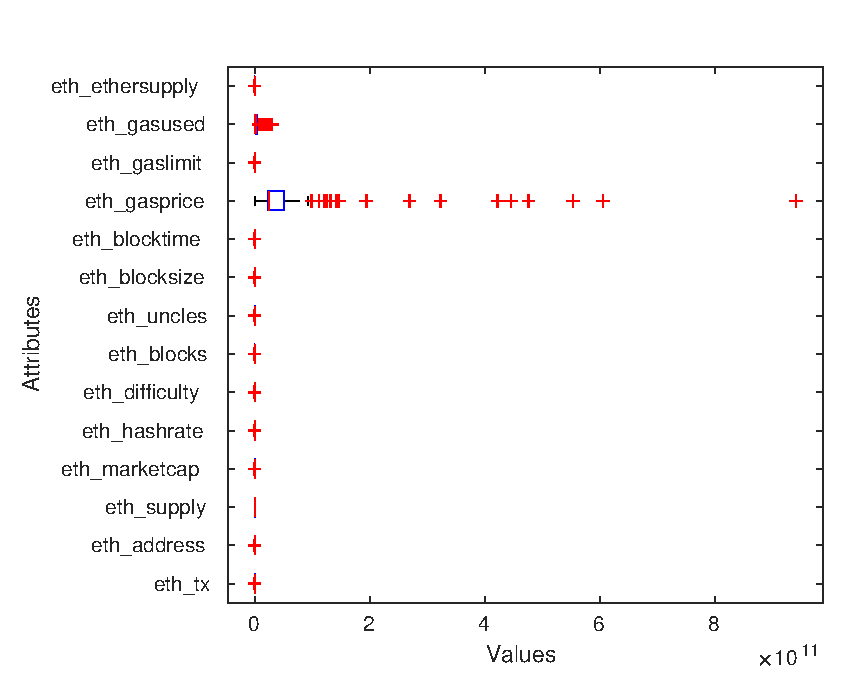
\includegraphics[scale = 0.9]{main/boxplot_before_norm.eps}
\end{figure}


Next, we visualize the distribution of the dataset after normalizing the columns. Note that we normalize each column in the dataset using the method that is used in that of the Boston Example provided by Peter Tino.

\begin{figure}[H]
\centering
\caption{Here is a boxplot of the 14 attributes that we are going to perform PCA on after they have been normalized, note that these are more suitable distributions to perform PCA on.}
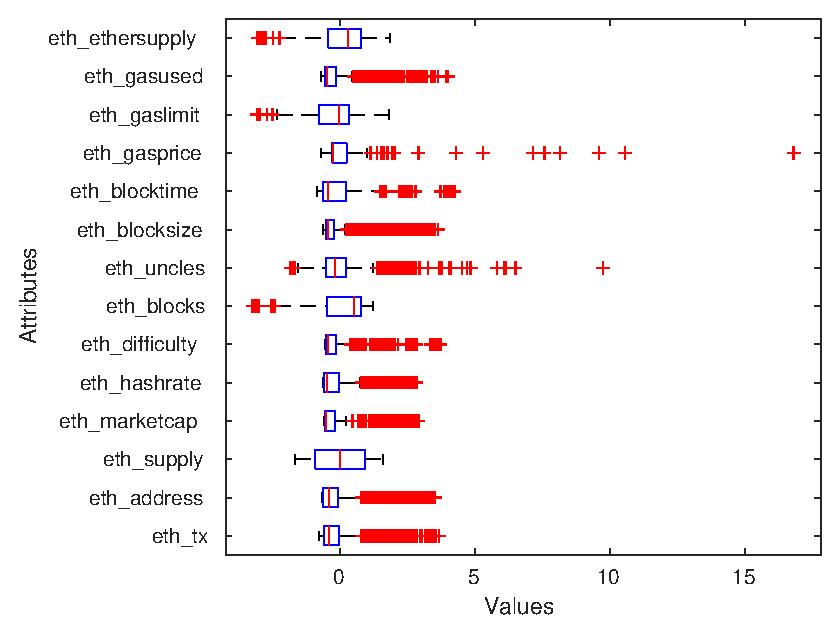
\includegraphics[scale = 0.9]{main/boxplot_after_norm.eps}
\end{figure}


\subsection{Labelling the Ether Price}
Next, we must label the price of Ether, we do this so that in the later stages we may visualize our PCA into some dimensional projection. Due to the interesting nature of this data set, we must use a slightly different labelling scheme. In order to better justify this scheme, we see a histogram of the \texttt{eth\_etherprice} column.

\begin{figure}[H]
\centering
\caption{Here is a histogram that allows us to visualize the Price of Ether, and the total number of occurences tha these prices happen. Note the right skew that we get from this graph}
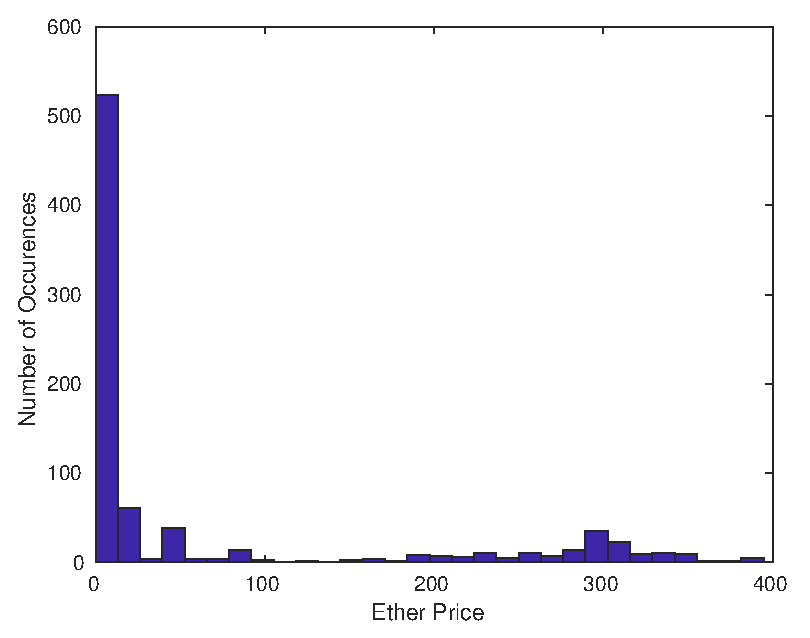
\includegraphics{main/eth_priceOnly_noYMax.eps}
\end{figure}

As we can see in the above histogram, the price of Ether is quite drastically skewed to the right. This can be explained in that Ethereum spent a great deal of its life below the $\$25$ mark, and sharply increased in price in the Summer of 2017. Now, because of the right skew of the data, we use a different labelling scheme. Our scheme is as follows:

\begin{center}
\begin{tabular}{ |c|c|c| } 
\hline
Ether Price p & Label & Value\\
\hline
$p < 25$ & Very Low & 1\\ 
$25 \leq p < 118.75$ & Low & 2\\ 
$118.75 \leq p < 212.5$ & Medium & 3\\ 
$212.5 \leq p < 306.25$ & High & 4\\ 
$p \geq 306.25$ & Very High & 5\\ 
\hline
\end{tabular}
\end{center}

By doing this, we are essentially considering the Ether Prices under 25 as one single block (Very Low), then we split up the remaining values into 4 remaining blocks. Thus, we end up with the following histogram for the Ether Price, note that in this diagram, the y axis has been limited to 100 (we already know it hits a high of around 500), so that we can better view the data.

\begin{figure}[H]
\centering
\caption{Here is a histogram showing the Prices of Ethereum with the Labels indicated by a Red Line, Please note that we have limited the y axis to be from 0 - 100, so that we can get a better view of the data}
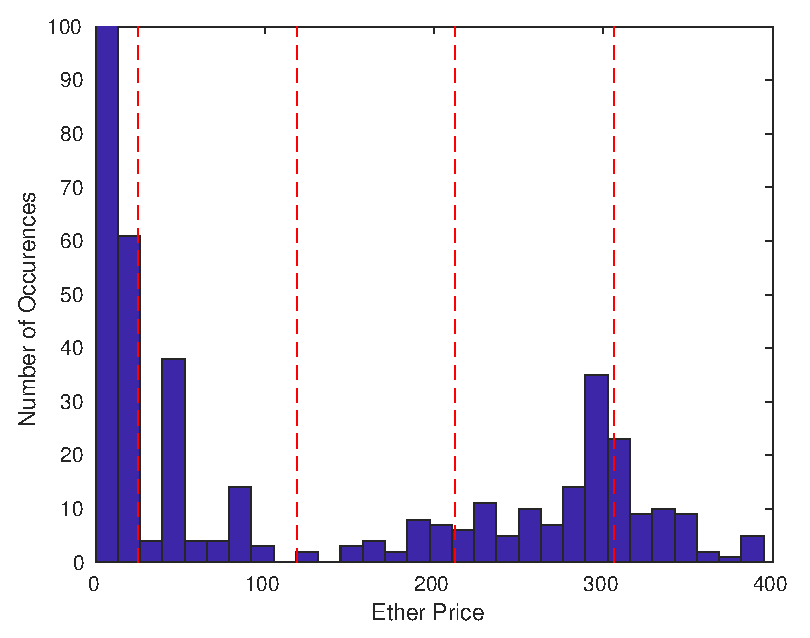
\includegraphics[scale=0.75]{main/eth_priceOnly.eps}
\end{figure}

\subsection{Principal Component Analysis}
Now that we have preprocessed our data into a single dataset, and a labelled attribute, we are ready to perform some PCA. The first step we take is to create a Covariance Matrix of our data. We do this through the \texttt{cov()} method that is provided in Matlab. This yields a $14$x$14$ matrix. 
\vspace{3mm}

Next, we calculate the eigenvectors and eigenvalues through the \texttt{eig()} method, again provided by Matlab. Once we have done this, we now have the ability to analyze our principal components. Here is a scree plot that we can use to visualize our eigenvalues. The bars represents the percentage of variance described  by only that principal component. Whereas the line shows us the cumulative variance described by each of the principal components in descending order.

\begin{figure}[H]
\centering
\caption{A Scree Plot Showing the Variance described by each eigenvector, up to the 8th Principal Component. The blue line shows the cumulative percentage variance described by the data, whereas the orange bars describe the percentage of variance described by that particular component. Note, we only show the first 8 principal components, as thet are so small.}
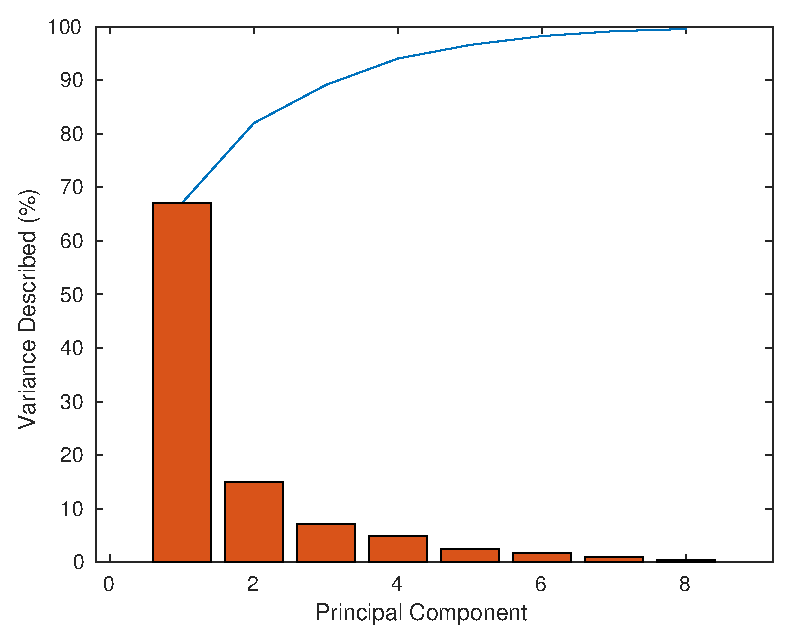
\includegraphics[scale = 0.75]{main/scree_plot.eps}
\end{figure}

Please note that in our Scree plot we are only considering the first 8 principal components because the components 9 - 14 are extremely small. In fact, from the first 8 components we are capturing 99.5342\% of the variation in the data. We want to project our data into the new space using some number of the principal eigenvectors. So, now we must choose this number, I have provided this table as it gives the exact percentages, as opposed to our Scree, which simply provides an overview.

\begin{center}
\begin{tabular}{ |c|c| } 
\hline
Principal Component & Cumulative Variance Present (\%) \\
\hline
1 & 67.04 \\ 
2 & 81.98 \\ 
3 & 89.12 \\ 
4 & 94.03 \\
\hline
\end{tabular}
\end{center}

We see that our first principal component is able to describe $67.04\%$ of the variance in our data, which is very high. Furthermore, our first two principal components are able to describe $81.98\%$ of the variance in our dataset. As we are able to hold over $80\%$ of our data from the first two components, it makes sense to project our data into its new space using the first two principle components .
\vspace{3mm}

We let $\bm{A}$ be the $825$x$14$ matrix storing our normalized data. Then, we let $\bm{B}$ be the $14$x$2$ matrix which we call our projection matrix. This projection matrix is the concatenation of the two eigenvectors with the largest eigenvalues. Thus we calculate the 2 dimensional projection of our data $\bm{P}$ by

$$
\bm{P} = \bm{A} \cdot \bm{B}
$$

Here is the 2D projection of our dataset into the the new subspace that is created by the first two principal components, first we show the legend which shows the labelling scheme.

\begin{figure}[H]
\centering
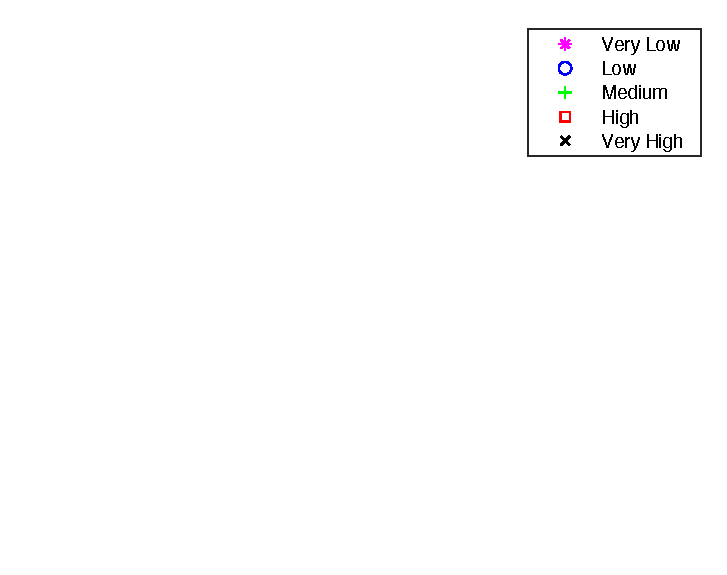
\includegraphics[scale = 0.7]{main/legend_2D_proj_copy.pdf}
\end{figure}
\begin{figure}[H]
\centering
\caption{Here is a projection of our original 14 dimensional dataset into the new 2 dimensional subspace under the labelling scheme on the Pricer of Ether that we have described earlier. We include the legend above.}
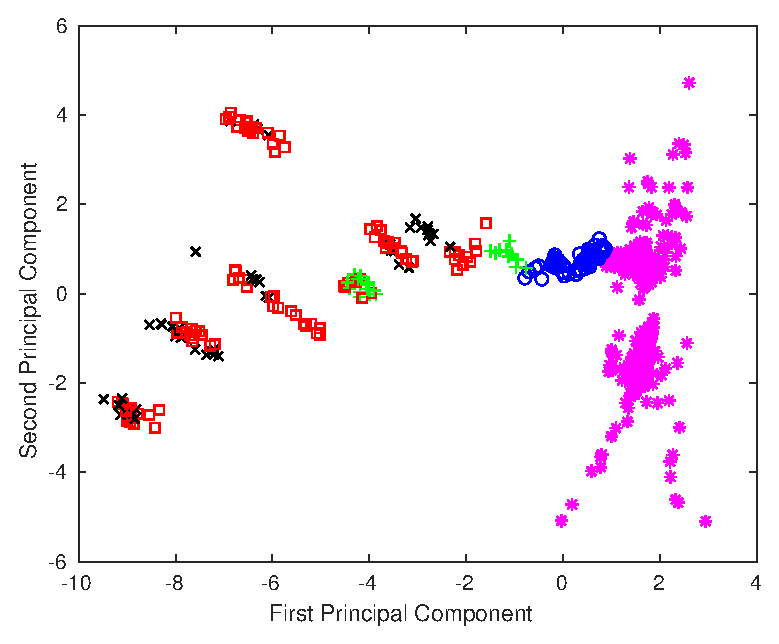
\includegraphics{main/eth_2d_projection.eps}
\end{figure}

As we might have expected, this 2D projection shows some very close clustering, as our scree plot might have suggested. This is down to the fact that we are able to capture over 80\% of the variance in our dataset in this new subspace. If we were to extend this and create a 3D plot, we could capture nearly 90\% of the variance in our data. This however is not necessary for the majority of this project as 81.98\% is very high for 2 dimensions. If the variance captured was lower, I would expect to see much less clustering. Another note is that we see the best clustering for the values labelled Very Low (the magenta stars), this is perhaps because this is the label that was put on the greatest number of points in our dataset. We also include a biplot for this PCA experiment, seen below.


\begin{figure}[H]
\centering
\caption{A Biplot of our original data projected into the new 2D subspace by the first two principal components. I have omitted the labels lines that are clustered to the left as they are too close to view. Here are the missing labels in order from highest to lowest in the y axis: \texttt{tx}, \texttt{gasused}, \texttt{gaslimit}, \texttt{address}, \texttt{marketcap}, \texttt{hashrate}, \texttt{blocksize}, \texttt{difficulty}.}
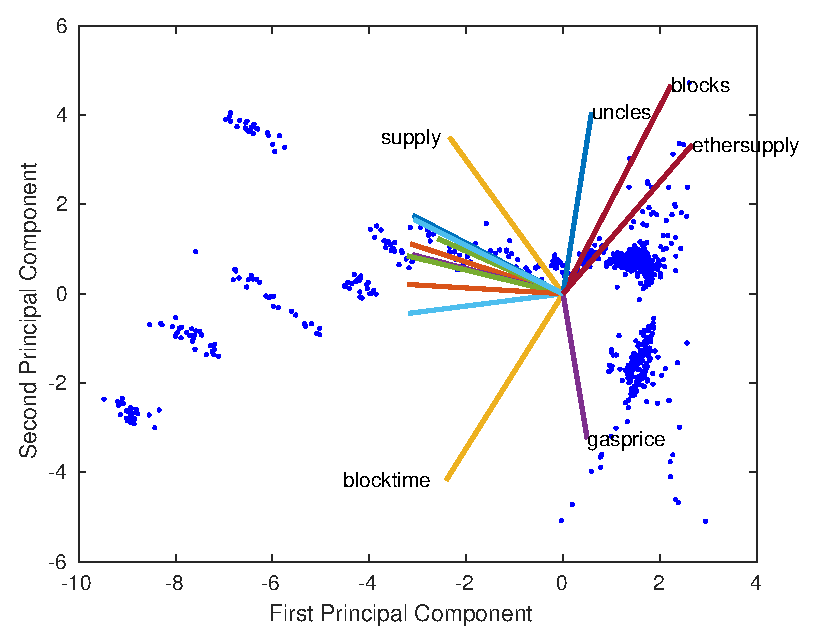
\includegraphics{main/eth_2d_biplot_better.eps}
\end{figure}

%%%%%%POTENTIALLY SERIOUSLY WRONG HERE, MIGHT NEED TO CHANGE THIS BIT%%%%%%%%
The biplot consists of all of our data points plotted in the new subspace, with the addition of 14 vectors. This allows us to visualize our data points, and the points in our eigenvector for each attribute. We note that the points to the right, in particular the ethersupply and blocks variables seem to play the largest role in the first principal component, note that these points are pointing north-west, and thus means that they played a large role in the second principal component. Perhaps this suggests that our \texttt{eth\_ethersupply} and \texttt{eth\_blocks} attributes provide a lot of the variance in our data. In fact, this is one of the reasons that I have chosen to perform my second PCA experiment on this attribute. It is also important to note that the vectors which appear close together are very closely related. In particular we note that out \texttt{eth\_marketcap} and \texttt{eth\_hashrate} attributes are very close together, and the vector is very small. There is likely to be a negative correlation between these two attributes for our dataset. This is to be expected, as the Ethereum marketcap often increases with time, and the Hash rate is becoming higher as time increases and mining Ether gets harder.
\vspace{3mm}

Here, we have projected our dataset into a new 3 dimensional subspace using the first three principal components, just out of curiosity, to see how it compares to the 2D projection. The 2D projection captures 81.98\% of the variance in our data, wheres, this 3D projection should capture 89.12\% of the variance in our dataset. Thus, we expect that this will not show a great deal more clustering than the 2D projection does. 

\begin{figure}[H]
\centering
\caption{Here is a 3D projection which is created from our first three principal components being concatenated into our 3x3 projection matrix. We then multiply this by our original data to view this projection on our labelling of Ether Price, these first 3 principal components allow us to capture 89.12\% of the variance in our data, which is extremely high. We do not need this 3D projection, we have just included it to see if we are able to visualize better any clustering in our data.}
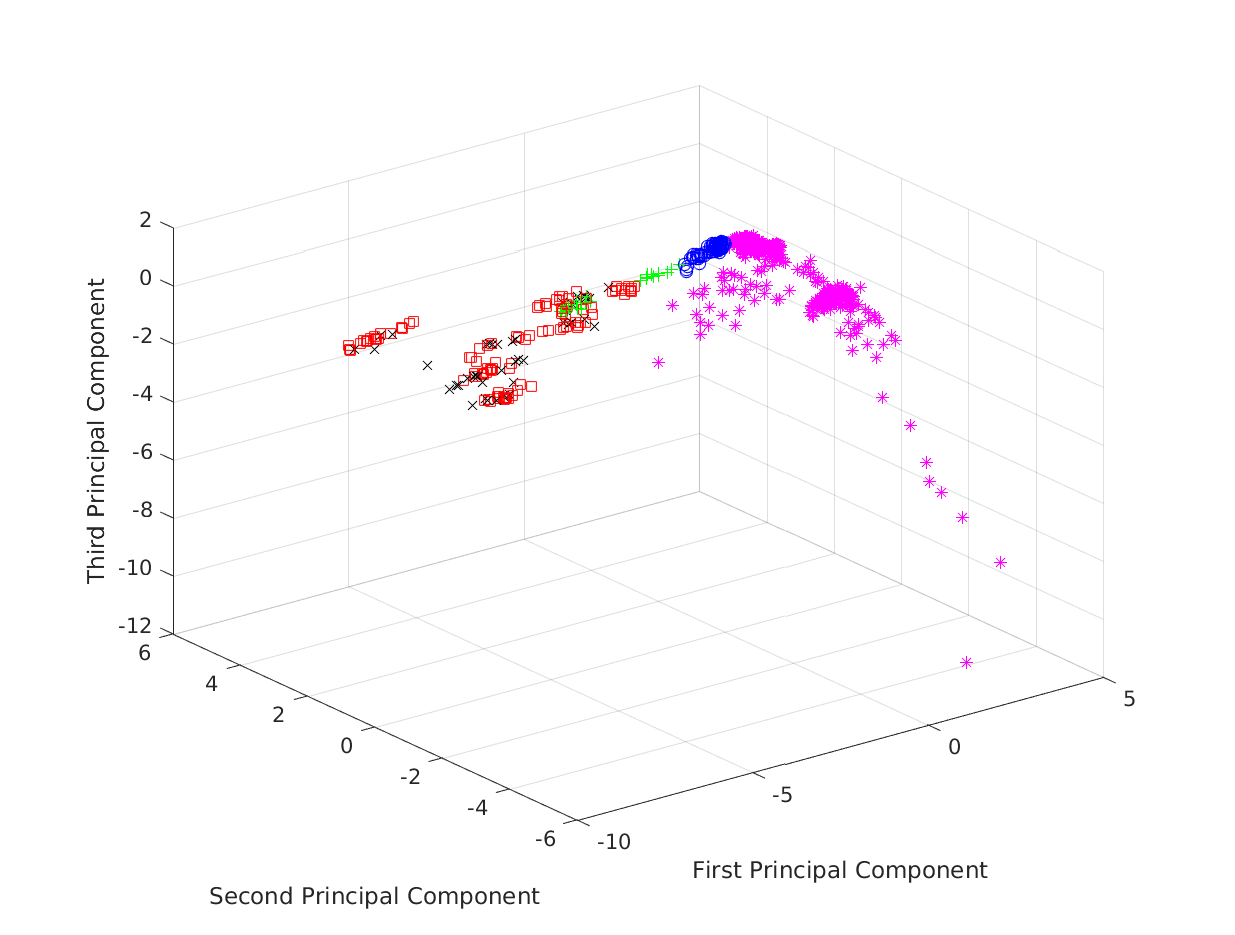
\includegraphics{main/eth_3d_projection.eps}
\end{figure}


 % It can be seen in Figure 5.  The direction and length of the
%vectors produced indicates the contribution to the principal components from each attribute.  The attributes to
%the right of the y-axis had the largest contribution to the first principle component, whilst those above the x-axis
%had larger contributions towards the second principle component.  Furthermore, vectors that are close to each
%other provide relationships.  For example,  it proves that total phenols is strongly related to proanthocyanins
%and flavinoids, which are what make up total phenols.  The nonflavanoidal phenols seem to contribute to the
%alkalinity of ash, and vice versa.  These were tested through some coordinate projections.


%%%%%%%%%%%%%%%%%%%%%%%%%%%%%%%%%%%%%%%%%%%%%%%%%
\section{Local Experiment Labelling Ether Supply}
A number of the attributes in our dataset can be used to describe how hard it is to currently mine Ether. This is the computationally intensive work, often performed by large machines with multiple Graphics Processing Units, which specifically is the validation of transactions within the Ethereum blockchain. By doing this the machines doing this work are rewarded fractions of Ether\cite{ethereum_info}. There are a number of interesting problems surrounding the creation of Ethereum, in particular the creation and circulation of too much Ether could potentially negatively effect the Ether market. In fact, it's developers intend on limiting the supply of Ether, and even destroying some. In this section, I will label the column \texttt{eth\_ethersupply}, which describes the new supply of Ether each day. 

%There are a number of interesting problems surrounding the creation of Ethereum, in particular the creation and circulation of too much Ether could potentially negatively effect the Ether market.

\subsection{Preprocessing our data}
In the previous experiment, we had to perform PCA on our data whilst excluding the \texttt{eth\_ens\_register} attribute, so in this section, we consider the subset of our original data in which that attribute has valid points. That is data collected between 08/05/2017 and 2/20/2018. Note, that the data I am using is being constantly updated and hence we have more current data with some information about 2018. Furthermore, we have deleted the attribute \texttt{eth\_supply}, due to its large correlation to the new supply of Ether daily. Thus, we are left with a dataset that has 287 instances of 14 attributes. 

As we saw in our previous experiment of the global dataset, it was clear that we had to normalize each attribute, the same must be true for this experiment. I have included a boxplot of all attributes to provide a comparison to that of our new variable \texttt{eth\_ens\_register}, and \texttt{eth\_etherprice}, which has been added back into our data. as before, we of course remove the attribute that we are labelling, which is \texttt{eth\_ethersupply}.

\begin{figure}[H]
\centering
\caption{A Boxplot visualizing the distribution of our 14 attributes, from the last boxplot, we have added the \texttt{eth\_ens\_register} and \texttt{eth\_etherprice} attributes. We have included all of the attributes which are duplicates from Figures 1 and 2 so that they can be compared to our new variables.}
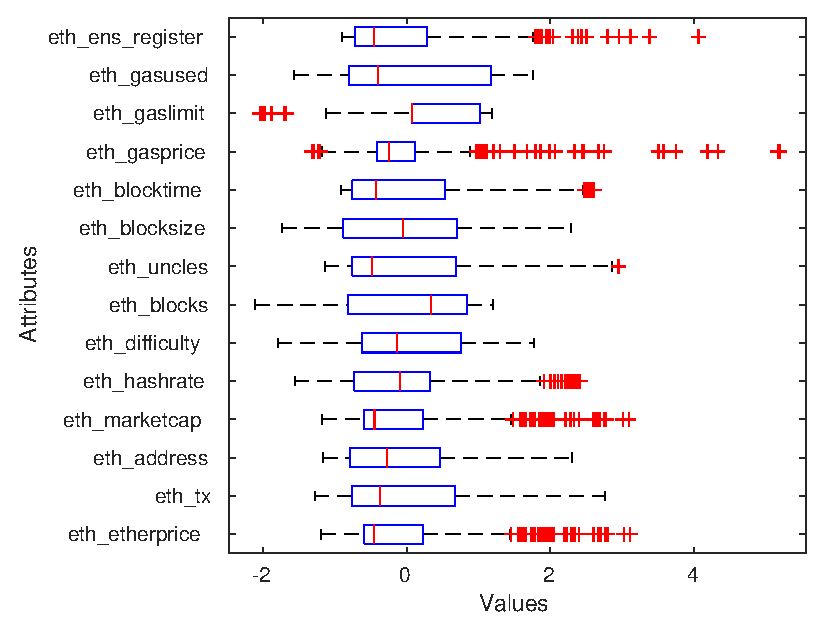
\includegraphics{local/boxplot_after_norm_supply.eps}
\end{figure}

\subsection{Labelling The Supply of Ether}
In this section, we aim to label the new supply of Ether per day in an appropriate manner. We chose the following labelling scheme:

\begin{center}
\begin{tabular}{ |c|c|c| } 
\hline
Ether Supply s & Label & Value\\
\hline
$s < 18350$ & Very Low & 1\\ 
$18350 \leq s < 22100$ & Low & 2\\ 
$22100 \leq s < 25850$ & Medium & 3\\ 
$ s \geq 25850$ & High & 4\\ 
\hline
\end{tabular}
\end{center}

Again, we plot a histogram of this data, so we can visualize its distribution. Note that we have added red Lines, which seperates the data into our seperate labels. This labelling scheme was chosen so that the first cluster is contained in the Very Low section. Then we split the remaining space of our graph into 3, then added a Line there to seperate them. We chose to call the term Very Low to describe the lowest number of New Ether supply as it is significantly lower than the rest of the data.

\begin{figure}[H]
\centering
\caption{Here is a histogram that we use to visualize the distribution of the Ether Supply Per Day, note that we visualize our labelling scheme by the four red lines appearing on the graph.}
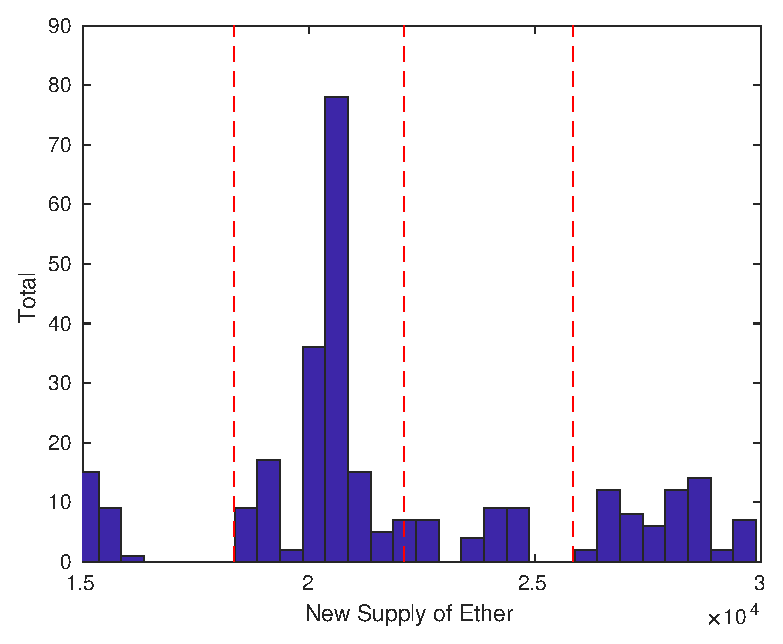
\includegraphics[scale=0.75]{local/eth_supplyOnly.eps}
\end{figure}

Now we have an appropriate labelling scheme and have preprocessed the data, we are now ready to perform the Principal Component Analysis.

\subsection{Principal Component Analysis}
In the previous section we performed the Principal Component Analysis on the global data, we will now do the same on our localized data. Please note that for these calculations, we use the same functions in Matlab as we did previously. We again create a Scree plot and we note that it is fairly similar to the Scree plot that was previously considered.

\begin{figure}[H]
\centering
\caption{A Scree Plot Showing the Variance described by each eigenvector, up to the 8th Principal Component. The blue line shows the cumulative percentage variance described by the data, whereas the orange bars describe the percentage of variance described by that particular component. Note, we only show the first 8 principal components, as thet are so small. This scree plot is different to that of the Scree of the First experiment as our data has changed, in particular we have a local view of our dataset and we have changed the attributes.}
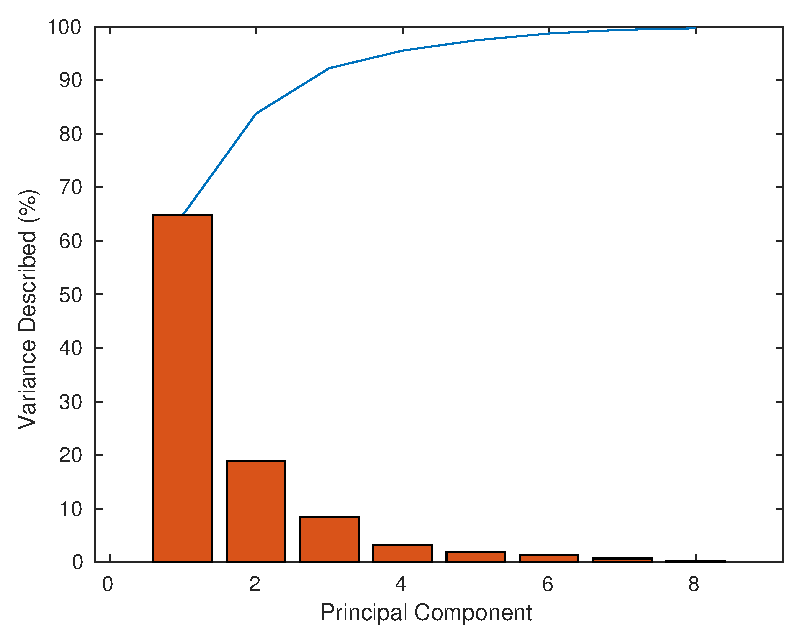
\includegraphics[scale = 0.75]{local/scree_plot_supply.eps}
\end{figure}

Here are the exact cumulative percentages as described by our Scree Plot for our first four principal components, to 2 decimal places.

\begin{center}
\begin{tabular}{ |c|c| } 
\hline
Principal Component & Cumulative Variance Present (\%) \\
\hline
1 & 64.79 \\ 
2 & 83.73 \\ 
3 & 92.23 \\ 
4 & 95.50 \\
\hline
\end{tabular}
\end{center}

We thus see that our first principal component again provides a great amount of detail about the variance of our dataset, however it tells us slightly less than the first principal component did in our global experiment. We also note that our second and third principal components are larger than in our first experiment. So overall, from our first two principal components we are able to view 83.79\% of our data. This is quite large, so again it makes sense for us to project our data using the first two principal components, as we will still be able to capture a lot about the data. We do the same calculations as before to calculate our 2d projections, except this time our 2D projection will have 297 points of data in our new space. We get the following projection:
\begin{figure}[H]
\centering
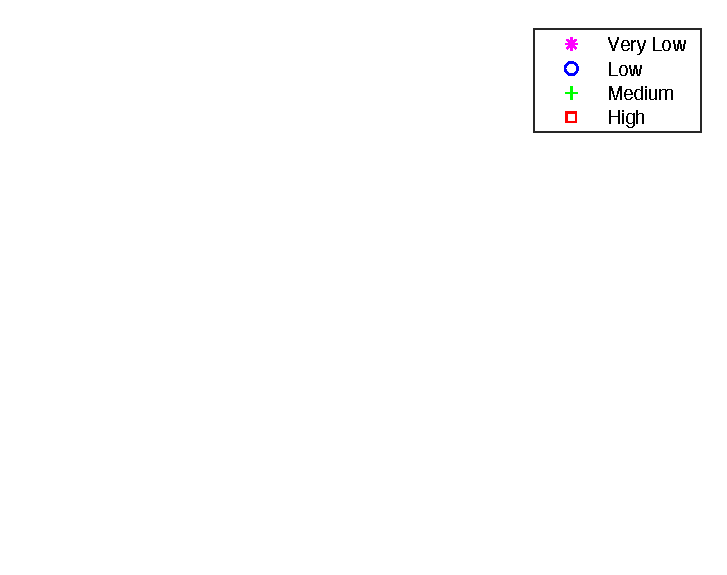
\includegraphics[scale = 0.7]{local/legend_2D_proj_copy.pdf}
\end{figure}
\begin{figure}[H]
\centering
\caption{Here is a projection of our original dataset into the new 2 dimensional subspace by the first two principal components calculated from the covariance matrix of our dataset.}
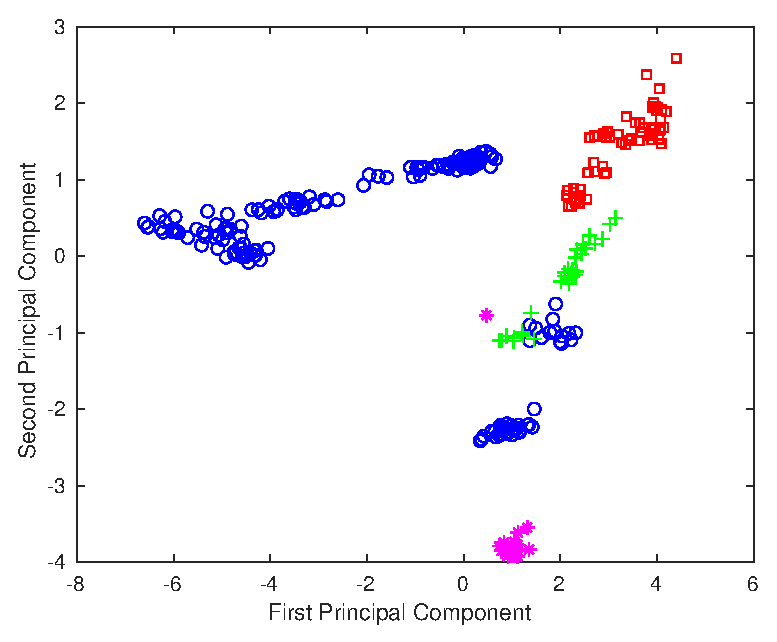
\includegraphics{local/eth_2d_projection_supply.eps}
\end{figure}

This 2D projection into our new subspace again shows some tight clusters. This is again due to the fact that this new subspace is able to capture such a high percentage of the variance in our dataset (83.73\%). However, in this case we do note that there are some outliers, for example there is a magenta asterisk(Very Low) at approximately $(0.5, 0.75)$. Furthermore, we notice the blue circles have one main cluster, and then two seperate clusters. We note that there are less instances of our dataset in this PCA experiment, perhaps if we had a larger dataset, the clustering might become a bit more apparent.

\begin{figure}[H]
\centering
\caption{A Biplot of our original data projected into the new 2D subspace by the first two principal components. I have omitted the labels lines that are clustered to the left as they are too close to view. Here are the missing labels in order from highest to lowest in the y axis: \texttt{gasused}, \texttt{tx}, \texttt{etherprice}, \texttt{marketcap}, \texttt{address}, \texttt{hashrate}, \texttt{gasprice}, \texttt{blocksize}, \texttt{gaslimit}.}
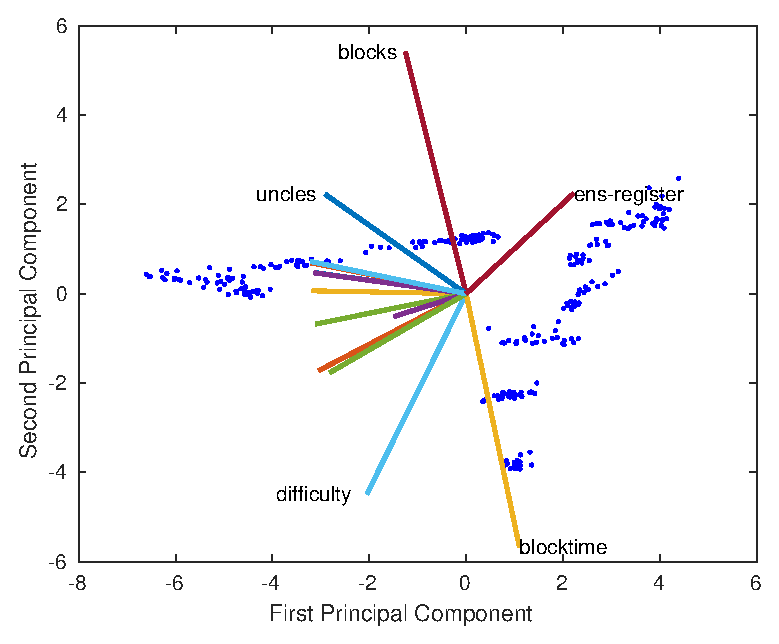
\includegraphics{local/eth_2d_biplot_supply.eps}
\end{figure}

From the biplot we see that the \texttt{eth\_blocks} attribute contributes greatly to the second principal component. We also see that the \texttt{eth\_ens\_register} attribute is significant in terms of the first and second principal component. Again we see an unsurprising result in that the \texttt{eth\_marketcap} and \texttt{eth\_etherprice} vectors are almost identical. This suggests a great correlation between the data of these attribute, which are clearly heavily linked.

\begin{figure}[H]
\centering
\caption{Here is a 3D projection which is created from our first three principal components being concatenated into our 3x3 projection matrix. We then multiply this by our original data to view this projection on our label of the Ether Supply, these first 3 principal components allow us to capture 92.23\% of the variance in our data, which is extremely high. We do not need this 3D projection, we have just included it to see if we are able to visualize better any clustering in our data.}
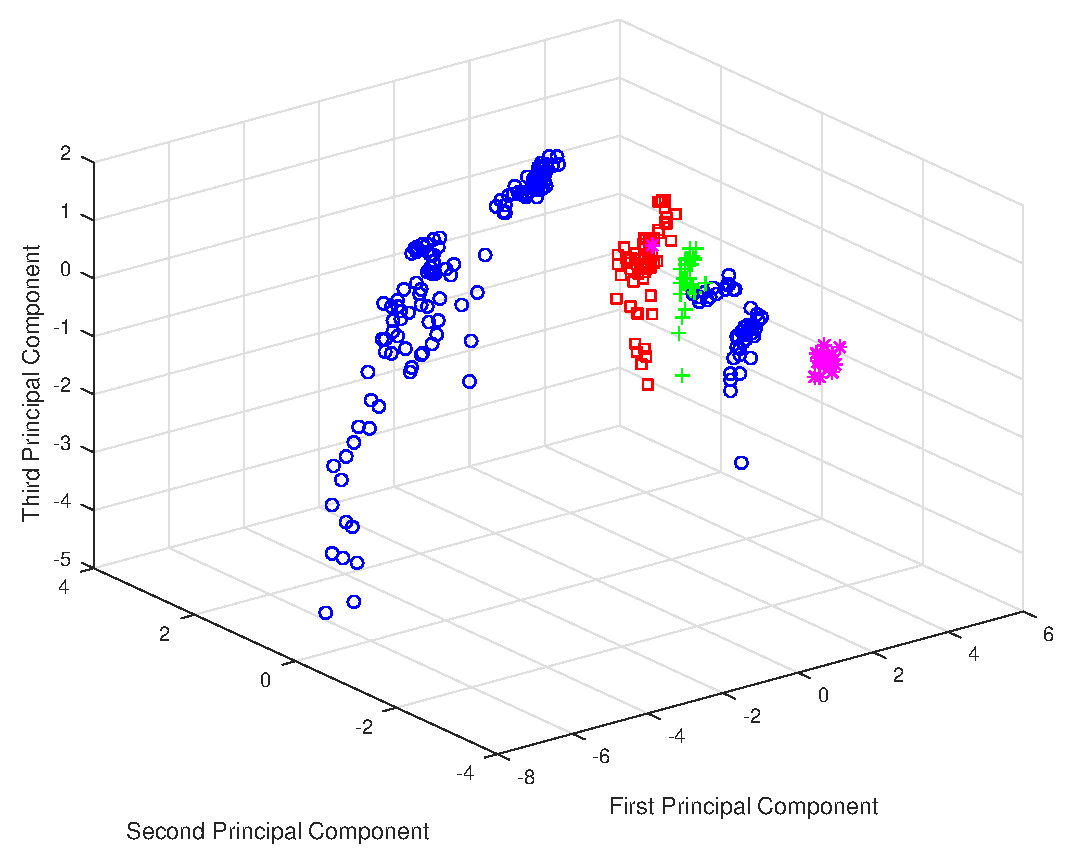
\includegraphics{local/supply_3d_projection.eps}
\end{figure}

%%%%%%%%%%%%%%%%%%%%%%%%%%%%%%%%%%%%%%%%%%%%%%%%%%%%%%%%%%%%%%%%%%%%%%%%%%%%%%%
\section{A Final Experiment on the Price of Bitcoin Using our Ethereum Dataset}

In the final PCA experiment for this project, I have chosen to extend the dataset that I am currently using. I have added the daily high market price of Bitcoin to the corresponding day that the Ethereum data was collected(The day is what connects these two dataset). I chose to use the high price, as opposed to the starting, low or closing price, I decided this for no particular reason, as for the purpose of this project it will not matter. The cryptocurrency markets can be extremely volatile, and it often is the case that if Bitcoin sees a sharp increase or decrease in market price, then the majority of the smaller coins will follow the same trend. Upon completion of this PCA experiment, perhaps we can compare our data projections to that of the Ether price, to see if our calculations on the Ethereum dataset will also provide a good tool to decrease the number of dimensions when we need to consider the price of Bitcoin, instead of Ether. First, we preprocess the data and label the Bitcoin price.

\subsection{Preprocessing the data}
Our preprocessing in this section is again extremely similar. We first get the Bitcoin Price data for the matching dates that our Ethereum data is taken from, in this case we are again considering a global view of the dataset. From the previous experiments, it is clear that we must again normalize our data. We do this using the same methods, and we include the following boxplot to again compare the distribution of our attributes again. We again note that because our data has been updated since the first global experiment, and we now consider all attributes except for \texttt{eth\_ens\_register}, thus we  are preprocessing a dataset of 927 instances, and 15 attributes.

\begin{figure}[H]
\centering
\caption{Here is a box plot that we use to visualize the distribution of our 15 attributes after they have been normalized. It is clear that we must normalize our data because of our previous experiments. Further, we note that we include all attributes in the box plot just so they can be better visualized or compared.}
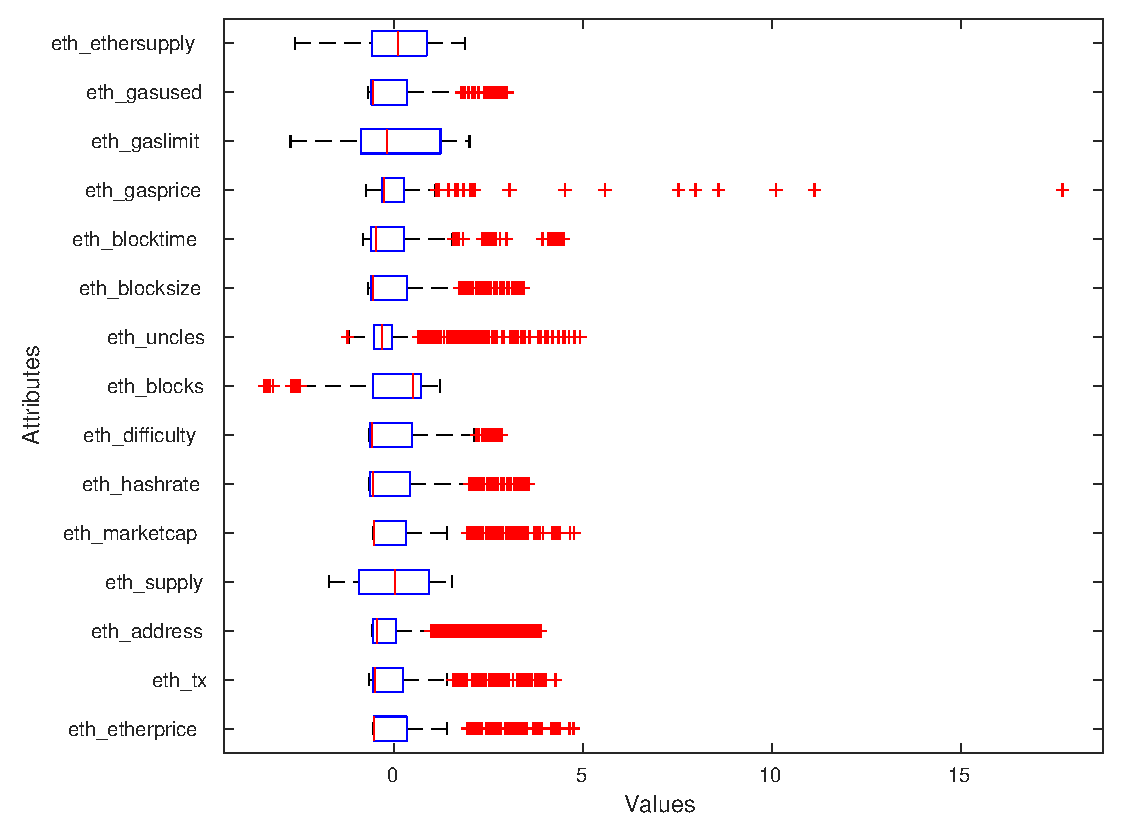
\includegraphics{final/boxplot_after_norm_btc.eps}
\end{figure}

Now, we label the the Bitcoin Price attribute.

\subsection{Labelling the Price of Bitcoin}
Here, we plot a histogram of all of our data points, so that we can visualize how the price of Bitcoin is distributed. We again notice a similar pattern that we have seen in the price of Ether, in that each attribute is skewed to the right. It is because of this that I have chosen to use a similar labelling scheme to the one that I used when labelling the \texttt{eth\_etherprice} attribute.

\begin{figure}[H]
\centering
\caption{Here is a basic histogram visualizing the distribution of the price of Bitcoin. It is noteworthy that our Bitcoin price is quite heavily skewed to the right.}
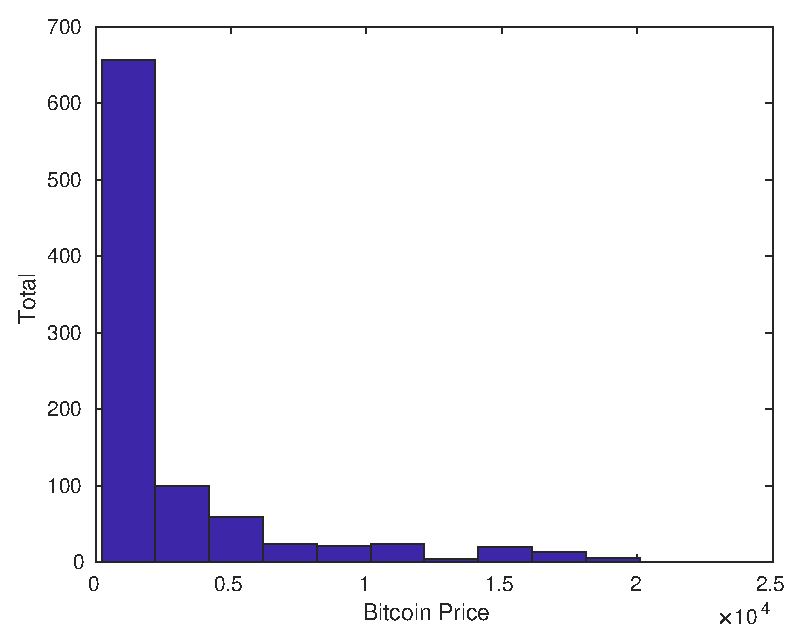
\includegraphics{final/btc_priceOnly.eps}
\end{figure}

From this box plot, we choose the following labelling scheme, note that as in our first Global experiment, we choose a very small first block, and then split up the remaining parts into three separate parts, due to the our data being skewed to the right.

\begin{center}
\begin{tabular}{ |c|c|c| } 
\hline
Bitcoin Price p & Label & Value\\
\hline
$p < 1500$ & Low & 1\\ 
$1500 \leq p < 7600$ & Medium & 2\\ 
$7600 \leq p < 14100$ & High & 3\\ 
$ p \geq 14100$ & Very High & 4\\ 
\hline
\end{tabular}
\end{center}

So, we end up with the following histogram, please note that we have limited the y axis between 0 and 60, so that we can get a better view of all of the data, we already seen in the previous graph how the total Number of occurrences for the Very Low Bitcoin prices reached over 600. So it is not important for us to visualize this again. We have added the labels as the red lines that appear on the graph. For the purpose of this experiment, from the histogram we see that it makes sense to seperate the data into four classes.

\begin{figure}[H]
\centering
\caption{Here is a Histogram showing the Price of Bitcoin with a y axis limited between 0 and 60, we do this to get a better view of the data, in the previous figure we saw the right skew of our dataset, so we do this so we can essentially zoom in on our data. We also include the labels described by the red lines to visualize our labelling scheme.}
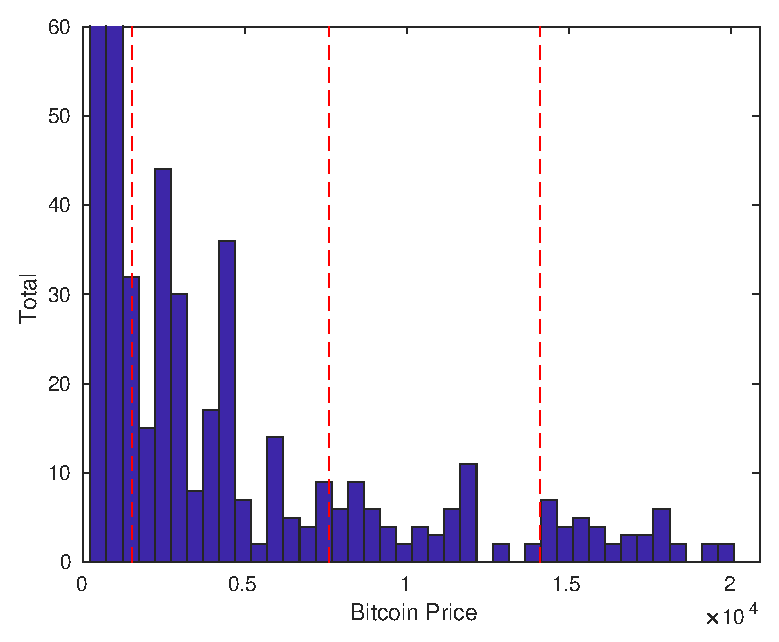
\includegraphics[scale=0.8]{final/btc_price_withLabel.eps}
\end{figure}

We have now labelled and preprocessed our data, so we are ready for the PCA.

\subsection{Principal Component Analysis}
As before, we perform the same steps by calculating the covariance matrix, and then the eigenvectors and eigenvalues, we then order the eigenvalues and their corresponding eigenvectors in descending order. We consider the eigenvector corresponding to the largest eigenvalue to be our first principal component. We end up with the following Scree Plot.

\begin{figure}[H]
\centering
\caption{A Scree Plot Showing the Variance described by each eigenvector, up to the 8th Principal Component. The blue line shows the cumulative percentage variance described by the data, whereas the orange bars describe the percentage of variance described by that particular component. Note, we only show the first 8 principal components, as thet are so small.}
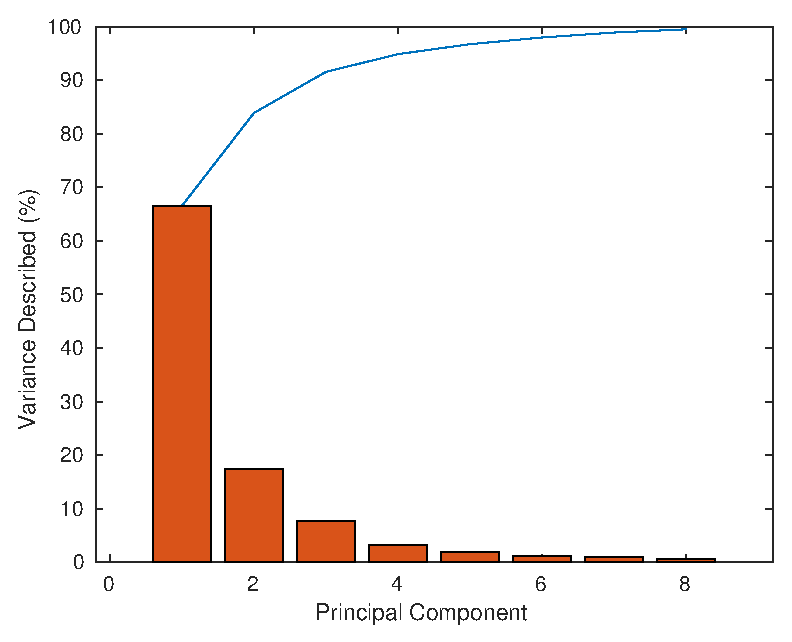
\includegraphics[scale = 0.75]{final/scree_plot_btc.eps}
\end{figure}

It is not surprising for us to get a similar result again, as the majority of our dataset has been consistent throughout this project. Here are the exact cumulative percent of variance of our first four principal components, as described above.

\begin{center}
\begin{tabular}{ |c|c| } 
\hline
Principal Component & Cumulative Variance Present (\%) \\
\hline
1 & 66.53 \\ 
2 & 83.88 \\ 
3 & 91.54 \\ 
4 & 94.84 \\
\hline
\end{tabular}
\end{center}

We see that the first two principal components describe 83.88\% of the variance in our data. Thus, we can project our data into a new subspace represented by two dimensions while still maintaining a lot of the variance in our data, that we don't want to lose. We end up with the following 2D projection of our data into this new subspace.
\begin{figure}[H]
\centering
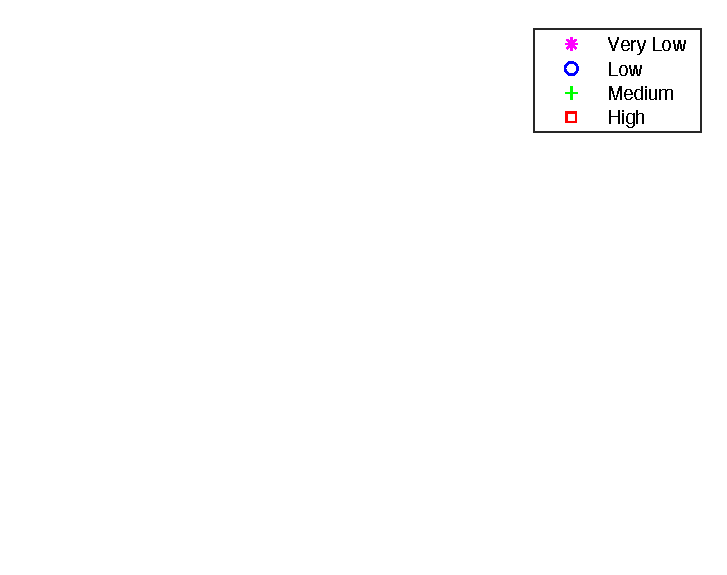
\includegraphics[scale = 0.7]{local/legend_2D_proj_copy.pdf}
\end{figure}
\begin{figure}[H]
\centering
\caption{Here is a projection of our original dataset into the 2 dimensional subspace as described by the first two principal components. Please see the legend above which describes our labelling scheme which we have used to label the price of Bitcoin}
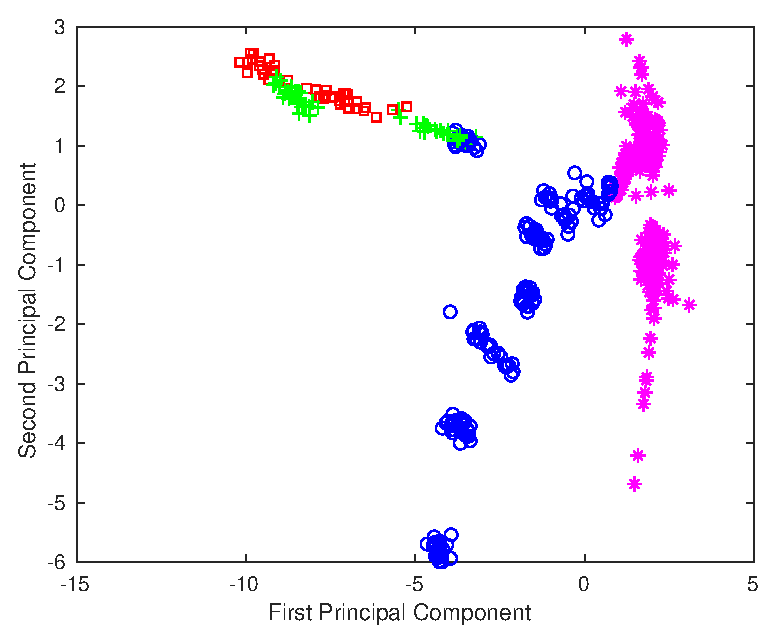
\includegraphics{final/btc_2d_projection.eps}
\end{figure}

We see some good clustering in this graph, in particular for the data points that are labelled as Very Low and High. 


\begin{figure}[H]
\centering
\caption{Here is a 3D projection which is created from our first three principal components being concatenated into our 3x3 projection matrix. We then multiply this by our original data to view this projection on our labelling of Ether Price, these first 3 principal components allow us to capture 89.12\% of the variance in our data, which is extremely high. We do not need this 3D projection, we have just included it to see if we are able to visualize better any clustering in our data.}
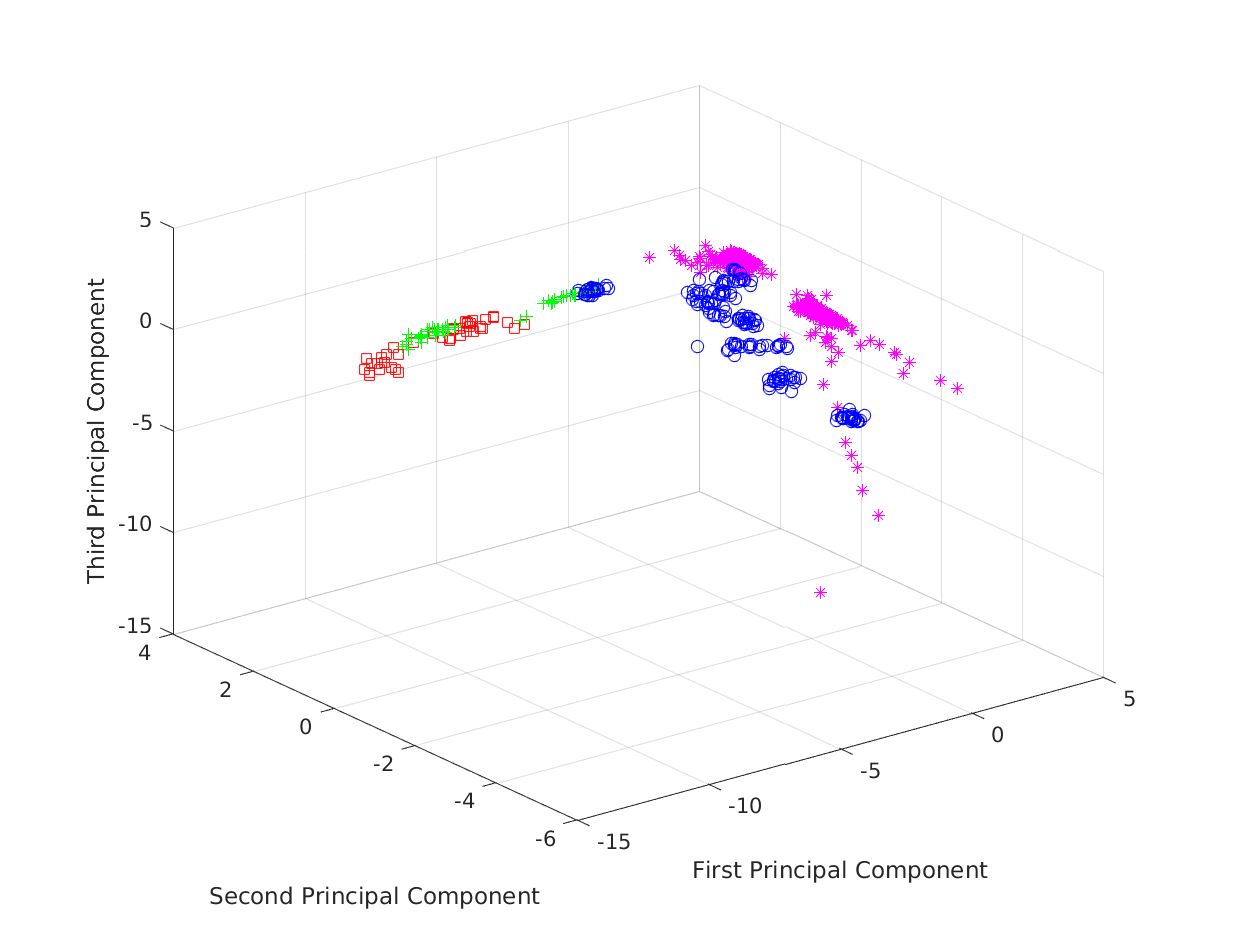
\includegraphics{final/btc_3d_projection.eps}
\end{figure}
 

\subsection{Comparison between First Global Experiment}
In this brief section, we will compare the projections of our datasets from the first and final PCA experiments into their own respective 2D subspaces. We note that in the first PCA experiment on Ether Price, we saw that it was appropriate to put Ether Price into 5 Labels. Thus, to make it a more appropriate comparison, we have redone the PCA with the following 4 Labels, which follows the same labelling criteria as the final PCA experiment did.

\begin{center}
\begin{tabular}{ |c|c|c| } 
\hline
Ether Price p & Label & Value\\
\hline
$p < 25$ & Low & 1\\ 
$25 \leq p < 150$ & Medium & 2\\ 
$150 \leq p < 275$ & High & 3\\ 
$ p \geq 275$ & Very High & 4\\ 
\hline
\end{tabular}
\end{center}

Here, we visualize the two resulting 2D projections next to each other. Please note that the data points are  not exactly the same due to the inclusion of the Ether price into the attributes considered for our PCA during the final experiment. Thus we notice that the subspace that we project our points into will be different.

\begin{figure}[H]
  \centering
  \begin{minipage}[b]{0.4\textwidth}
    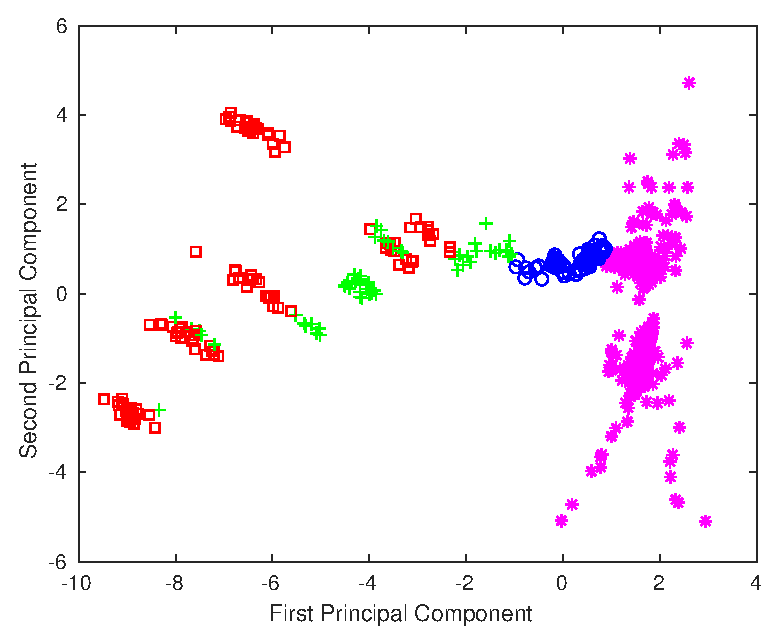
\includegraphics[width=\textwidth]{main/eth_2d_projection_4Labels.eps}
    \caption{A 2D Projection of Ether Price into the 2D subspace provided from the first PCA experiment, but with only 4 labels.}
  \end{minipage}
  \hfill
  \begin{minipage}[b]{0.4\textwidth}
    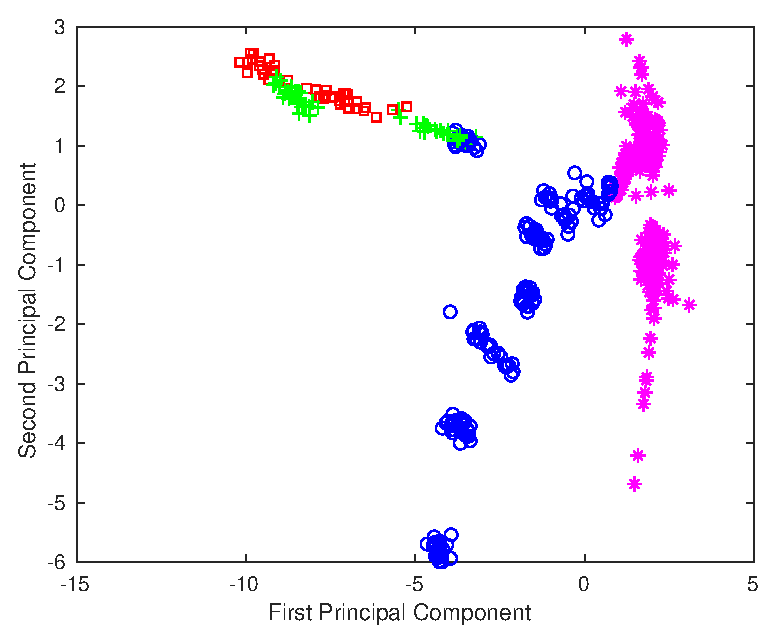
\includegraphics[width=\textwidth]{final/btc_2d_projection.eps}
    \caption{The 2D projection of our data into the new subspace as seen in the final PCA experiment above.}
  \end{minipage}
\end{figure}

We notice that the greatest similarities are between that of the Very Low/Low labels, and we can see some similarities between the two graphs. 

\section{Conclusion}
Having performed these three seperate PCA experiments on our dataset, we have seen some very good clustering in our 2D projections. This is because the variation in this dataset that is captured from the 2 dimensions of our new subspace have all been extremely high. We saw that we often had greater clustering when we had a higher number of instances of our dataset, as we have seen slightly less clustering in the second PCA experiment on the Supply of Ether. Perhaps, by doing further PCA experiments we could take a deeper look into this.

\begin{thebibliography}{9}
\bibitem{dataset} 
SRK 
Cryptocurrency Historical Prices,
\\\url{https://www.kaggle.com/sudalairajkumar/cryptocurrencypricehistory}
\\Last Used: 24/02/2018
 
\bibitem{ethereum_info} 
Useful Information on Ethereum,
\\\url{https://blockgeeks.com/guides/ethereum}
\\Last Used: 24/02/2018

\bibitem{pca_components}
Interpretation of the Principal Components,
\\\url{https://onlinecourses.science.psu.edu/stat505/node/54/}
\\Last Used: 24/02/2018


\end{thebibliography}

\end{document}

%%%%%%%%%%%%%%%%%%%%%%%%%%%%%%%%%%%%%%%%%%%%%%%%%%%%%%%%%%%%%%%%%%%%%%%%%%%%%%%%%%%%%%%%5

% Useful links : 

% DATASETS :
%     - https://www.kaggle.com/sudalairajkumar/cryptocurrencypricehistory

% FOR INFO ON Ethereum :
%     - blockgeeks.com/guides/ethereum

% For info on analysing eigenvectors
% https://onlinecourses.science.psu.edu/stat505/node/54
